\begin{frame}{Large Scale Viscous Flow Features (VFFs)}
    \begin{block}<+->{Glacier-like features (GLFs)}
        \begin{itemize}
            \item Lowest-order feature.
            \item Cirque-like alcoves and small valleys.
            \item Adjacent to LDAs.
        \end{itemize}
    \end{block}

    \begin{block}<+->{Lobate debris aprons (LDAs)}
        \begin{itemize}
            \item Converge/coalesce into LVFs.
            \item Convex downslope.
            \item Rough surface (ridge-and-furrow).
            \item From alcoves, craters, valleys and massif walls.
            \item Lobate terminus.
        \end{itemize}
    \end{block}
\sidecite{(\cite{Levy10,Brough16,Wueller25})}
\end{frame}
\begin{frame}{Large Scale Viscous Flow Features (VFFs)}
    \begin{block}<+->{Lineated valley fills (LVFs)}
        \begin{itemize}
            \item At valleys, canyons and confined spaces.
            \item Exhibit transverse and parallel flow lineations.
        \end{itemize}
    \end{block}
    \begin{block}<+->{Concentric crater fills (CCFs)}
        \begin{itemize}
            \item Contain concentric lineations.
            \item Fill crater.
            \item Associated with LDAs and LVFs.
        \end{itemize}
    \end{block}
\sidecite{(\cite{Levy10,Brough16,Wueller25})}
\end{frame}

\begin{frame}[label=LargeVFFs]{Large Scale Viscous Flow Features (VFFs)}
    \begin{figure}
        \centering
        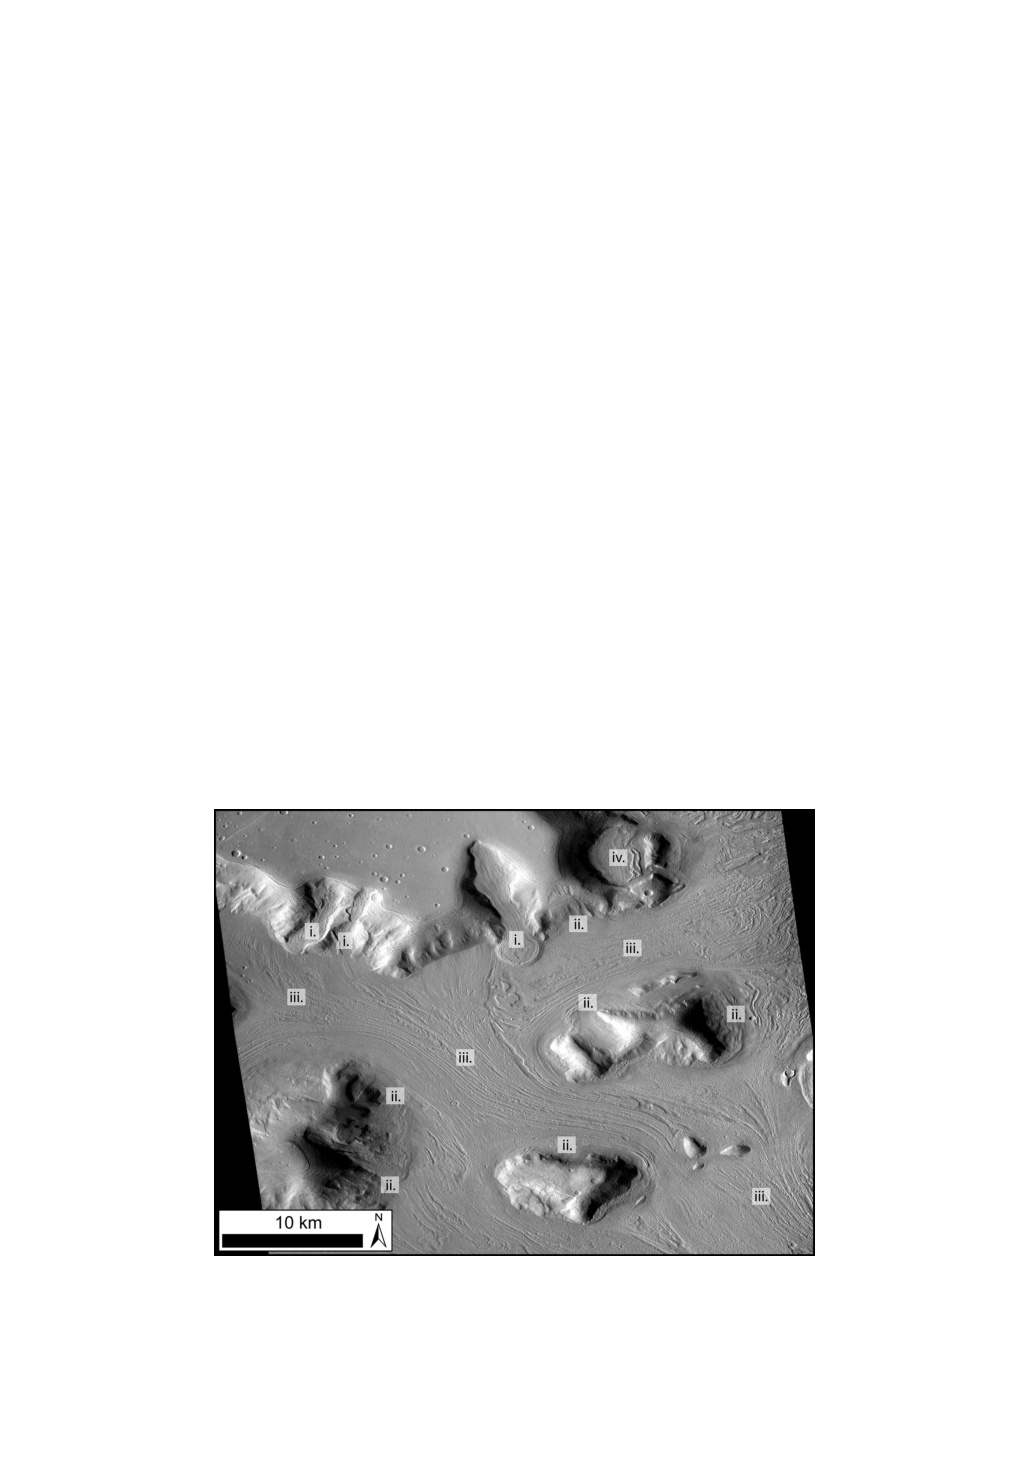
\includegraphics[
        width=\linewidth,
        height=0.65\textheight,
        keepaspectratio
    ]{Figures/Diagrams/Brough16_Fig1.pdf}
    \caption{CTX image data showing (i) GLFs; (ii) LDAs; (iii) LVFs; and (iv) CCFs at Protonilus Mensae ($42.62^{\circ}$N, $50.51^{\circ}$E; Figure from \cite{Brough16}).}
    \end{figure}
\end{frame}